\chapter{Wstęp}
Celem niniejszej pracy jest implementacja aplikacji mobilnej służącej do sterowania robotem minisumo. W ramach pracy dyplomowej powstał samodzielnie wykonany dwukołowy robot w pełni spełniający wymagania do startu w zawodach minisumo. Dodatkowo powstała aplikacja mobilna na platformę iOS, która daje możliwość obsługi oraz konfiguracji wyżej wspomnianego robota. Dzięki niej użytkownik może wybrać jedną z wielu strategii walki, ustalić maksymalną moc silników oraz uwzględnić oczekiwanie na start za pomocą odbiornika fal podczerwonych. Dodatkowo aplikacja oferuje możliwość zdalnego sterowania robotem za pomocą akcelerometru lub wirtualnego dżojstiku oraz sprawdzenia poprawności działania sensorów i silników. 

\section{Minisumo}
Minisumo jest jedną z kategorii walk robotów wzorowanych na popularnym japońskim sporcie – zapasach sumo. Tak samo jak i w prawdziwym sporcie, starcie odbywa się na okrągłym ringu. Wygrywa ten robot, który jako pierwszy wypchnie rywala z areny. Obowiązujące zasady są takie same dla każdej z kategorii (sumo, minisumo, nanosumo, pentosumo) z wyjątkiem dopuszczalnej wagi oraz rozmiaru. Dla minisumo maksymalna waga to 500 gramów, a szerokość oraz długość nie mogą przekroczyć 100 milimetrów. Dodatkowo każdy z robotów musi spełniać 
poniższe wymagania:
\begin{itemize}
\item musi być w pełni autonomiczny,
\item nie może być przytwierdzony do areny,
\item nie może zakłócać sterowania przeciwnika,
\item musi posiadać na wyposażeniu moduł startowy, dający możliwość zdalnego uruchomienia robota przez sędziego,
\item nie może emitować cieczy, gazów oraz nadmiernego ciepła.
\end{itemize}

Na rysunku ~\ref{fig:sumo_competitions} przedstawiono przykładową walkę robotów klasy sumo. Warto zauważyć, iż  wnętrze areny jest czarne, natomiast obwód biały. Dzięki zastosowanemu kontrastowi robot wyposażony w odpowiednie czujniki jest w stanie wykryć brzeg areny.

\begin{figure}[H]
	\centering
		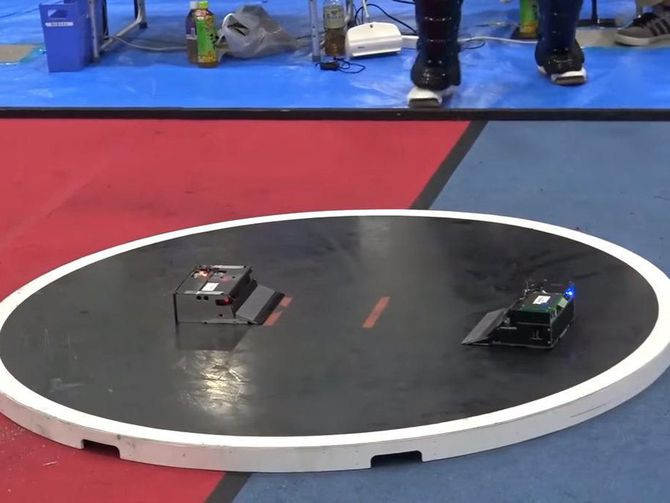
\includegraphics[width=0.75\linewidth]{pic01/sumo_competitions.jpg}
	\caption{Zawody sumo.}
	\label{fig:sumo_competitions}	
\end{figure}

\section{Założenia}
Główne założenia realizowanego projektu:
\begin{itemize}
\item stworzenie robota spełniającego wymagania kategorii minisumo,
\item sprawna sensoryka pozwalająca na wykrycie przeciwnika oraz końca ringu,
\item w pełni działająca komunikacja między robotem a aplikacją,
\item aplikacja mobilna pozwalająca na konfigurację wyżej wspomnianego robota.
\end{itemize}

Etapy realizacji wyżej wymienionych założeń zostały opisane w dalszej części pracy z podziałem na tworzonego robota minisumo oraz aplikację mobilną.
